\chapter{Proposed Attacks}

\section{Preimage Attack for $2$ Rounds of Round Reduced \KECCAK-$384$}

In this section, we present a preimage attack for a round reduced \KECCAK{}. We will show that the preimage can be found in $2^{88}$ time and $2^{87}$ memory for $2$ rounds of round-reduced \Keccak-$384$. Although it is not a practical attack, but it is an improvement over the existing best attack, for $2$ rounds of \Keccak-$384$, which takes $2^{129}$ time~\cite{guo2016linear}.


\subsection{Notations and Observations}
In the analysis, we will represent a state by the lanes. There are in total $5\times 5$ lanes. Each lane in a state will be represented by a variable which is a $64$-bit array. 
A variable with a number in round bracket $``( . )"$ represents the shift of the bits in array towards MSB. A variable with a number in square bracket $``[ . ]"$ represents the bit value of the variable at that index. If there are multiple numbers in the square bracket then it represents the corresponding bit values.

%% More details

We are going to use the following observations in our analysis.
\begin{enumerate}
\item \label{ob1}\textbf{Observation 1:} The $\chi$ is a row-dependent operation. Guo \etal in~\cite{guo2016linear}, observed that if we know all the bits of a row then we can invert $\chi$ for that row. It is depicted in the Figure~\ref{chi_inv}.
%------------------------------------------------------
\begin{figure}
\begin{center}
\begin{tikzpicture}[ampersand replacement=\&]
\matrix (m1) [matrix of nodes,
nodes={inner sep=5pt,text width=0.5cm,align=center,minimum height=.5cm, draw,text height=1em,text depth=.2em}
]{
	$a_0$ \& $a_1$\& $a_2$ \& $a_3$ \& $a_4$\\
};

\matrix (m2) [right = 1.2cm of m1, matrix of nodes,
nodes={inner sep=5pt,text width=0.5cm,align=center,minimum height=.5cm, draw,text height=1em,text depth=.2em}
]{
	$a_0^\prime$ \& $a_1^\prime$\& $a_2^\prime$ \& $a_3^\prime$ \& $a_4^\prime$\\
};
\draw[->, very thick] (m1)-- node[above, pos=0.5] {$\chi^{-1}$} (m2);
\end{tikzpicture}
\end{center}
\caption{Computation of $\chi^{-1}$ for full row \label{chi_inv}}
\end{figure}
%------------------------------------------------------
% check it for correctness
\begin{align}
a_i^\prime = a_i \oplus \left( a_{i+1} \oplus 1\right) \cdot \left( a_{i+2} \oplus \left( a_{i+3} \oplus 1 \right) \cdot a_{i+4}\right)
\end{align}


\item \label{ob2}\textbf{Observation 2:} When only one output bit is known after $\chi$ step, then the corresponding input bits have $2^4$ possibilities. Kumar \etal\cite{kumar2018cryptanalysis} gave a way to fix the first output bit to be the same as input bit and the second bit as $1$. It is shown in the Figure~\ref{chi_inv2}.

%------------------------------------------------------
\begin{figure}[ht]
\begin{center}
\begin{tikzpicture}[ampersand replacement=\&]
\matrix (m1) [matrix of nodes,
nodes={inner sep=5pt,text width=0.5cm,align=center,minimum height=.5cm, draw,text height=1em,text depth=.2em}
]{
	$a_0$ \& $*$ \& $*$ \& $*$ \& $*$\\
};

\matrix (m2) [right = 1.2cm of m1, matrix of nodes,
nodes={inner sep=5pt,text width=0.5cm,align=center,minimum height=.5cm, draw,text height=1em,text depth=.2em}
]{
	$a_0$ \& $1$ \& $*$ \& $*$ \& $*$\\
};
\draw[->, very thick] (m1)-- node[above, pos=0.5] {$\chi^{-1}$} (m2);
\end{tikzpicture}
\end{center}
\caption{Computation of $\chi^{-1}$ when only 1-bit is known in row \label{chi_inv2}}
\end{figure}

\item \label{ob3}\textbf{Observation 3:} Guo \etal in~\cite{guo2016linear} observed that when $4$ out of $5$ output bits are known after $\chi$ step then we can establish $4$ linear equations on the input bits of $\chi$.

$a_0, a_1, a_2, a_3, a_4$ are the output bits of $\chi$ and $a_0^\prime, a_1^\prime, a_2^\prime, a_3^\prime, a_4^\prime$ are the input bits.
\begin{align}
a_0^\prime = a_0 \oplus \left( a_{1} \oplus 1\right) \cdot \left( a_{2} \oplus \left( a_{3} \oplus 1 \right) \cdot a_{4}\right)
\end{align}
\begin{align}
a_1^\prime = a_1 \oplus \left( a_{2} \oplus 1\right) \cdot \left( a_{3} \oplus \left( a_{4} \oplus 1 \right) \cdot a_{0}\right)
\end{align}
\begin{align}
a_2^\prime = a_2 \oplus \left( a_{3} \oplus 1\right) \cdot \left( a_{4} \oplus \left( a_{0} \oplus 1 \right) \cdot a_{1}\right)
\end{align}
\begin{align}
a_3^\prime = a_3 \oplus \left( a_{4} \oplus 1\right) \cdot \left( a_{0} \oplus \left( a_{1} \oplus 1 \right) \cdot a_{2}\right)
\end{align}
\begin{align}
a_4^\prime = a_4 \oplus \left( a_{0} \oplus 1\right) \cdot \left( a_{1} \oplus \left( a_{2} \oplus 1 \right) \cdot a_{3}\right)
\end{align}

If we have values of $a_0, a_1, a_2, a_3$, then we have above $5$ equations in terms of the unknown output bit i.e. $a_4$. Then we can establish $4$ linear equations by eliminating $a_4$ from the above $5$ equations.

%------------------------------------------------------
\end{enumerate}


\subsection{Description of the Attack}
The \Keccak-{384} outputs $384$ bits hash value, which is represented by the first $6$ lanes in the state obtained at the end of the squeezing phase. The diagram in the Figure~\ref{initial_sq} represents this state. The values of remaining lanes are represented by $\star$ and we do not care these values. We are interested in finding a preimage for which $6$ lanes of corresponding state matches. We will call this state as \emph{final state}.
%------------------------------------------------
\begin{figure}[ht]
\begin{center}
\begin{tikzpicture}[ampersand replacement=\&]
\matrix (sm1) [matrix of nodes,
nodes={inner sep=5pt,text width=0.5cm,align=center,minimum height=.5cm, draw,text height=1em,text depth=.2em}
]{
	$\star$ \& $\star$\& $\star$ \& $\star$ \& $\star$\\
	$\star$ \& $\star$\& $\star$ \& $\star$ \& $\star$\\
	$\star$ \& $\star$\& $\star$ \& $\star$ \& $\star$\\
	$h_5$ \& $\star$\& $\star$ \& $\star$ \& $\star$\\
	$h_0$ \& $h_1$\& $h_2$ \& $h_3$ \& $h_4$\\
};
\node[] at (-1.7,-2.5) { 0 };
\node[] at (-0.85,-2.5) { 1 };
\node[] at (0.0,-2.5) { 2 };
\node[] at (0.9,-2.5) { 3 };
\node[] at (1.8,-2.5) { 4 };
\draw[thick,->] (-1.5, -3.2) -- node [above] {$x$} (0.0, -3.2);
\node[] at (-2.5,-1.5) { 0 };
\node[] at (-2.5,-0.75) { 1 };
\node[] at (-2.5,0.0) { 2 };
\node[] at (-2.5,0.8) { 3 };
\node[] at (-2.5,1.5) { 4 };
\draw[thick,->] (-3, -0.7) --  (-3, 0.8);
\node[] at (-3.3, 0) {$y$};
\end{tikzpicture}
\end{center}
\caption{The Final Hash State for \KECCAK-$384$ \label{initial_sq}}
\end{figure}
%------------------------------------------------
Furthermore, we can ignore the {$\iota$} step without the loss of generality, as it does not affect the procedure of the attack. However it should be taken into account while implementing the attack.

We further note that the initial state, which is fed to \Keccak-$f$ function, is the first message block which is represented by $25-2\cdot 6$ i.e., $13$ lanes. The remaining $12$ lanes are initially set to $0$. Pictorially, this state is represented by the diagram in the Figure~\ref{initial_state}. We call this state \emph{initial state}.
Our aim is to find the values of $a_0, a_1, a_2$, $b_0, b_1, b_2$, $c_0, c_1, c_2$, $d_0, d_1$ and $e_0, e_1$ variables in the initial state which lead to a final state having first six lanes as $h_0, h_1, h_2,h_3, h_4$ and $h_5$. 

We follow the basic idea of the attack, as given in the paper~\cite{naya2011practical}.
We start the attack by setting variables in the initial state which ensures zero column parity. 
This is done by imposing the following restrictions.
\begin{align}\nonumber
a_2 &= a_0 \oplus a_1,\quad b_2 = b_0 \oplus b_1, \quad c_2 = c_0 \oplus c_1\\ \label{cond_state1}
d_1 & = 0,\quad d_0 = 0\;\;\text{ and }\;\; e_1 = e_0. 
\end{align}

\begin{figure}
\begin{center}
\begin{tikzpicture}[ampersand replacement=\&]
\matrix (sm1) [matrix of nodes,
nodes={inner sep=5pt,text width=0.5cm,align=center,minimum height=.5cm, draw,text height=1em,text depth=.2em}
]{
	$0$ \& $0$\& $0$ \& $0$ \& $0$\\
	$0$ \& $0$\& $0$ \& $0$ \& $0$\\
	$a_1$ \& $b_1$\& $c_2$ \& $0$ \& $0$\\
	$a_2$ \& $b_2$\& $c_1$ \& $d_1$ \& $e_1$\\
	$a_0$ \& $b_0$\& $c_0$ \& $d_0$ \& $e_0$\\
};
\end{tikzpicture}
\end{center}
\caption{Setting of Initial State in the Attack\label{initial_state}}
\end{figure}
%--------------------------------------------------------
This type of assignment to the initial state will make the {$\theta$} step mapping, an identity mapping. Even though we have put some restrictions to the initial state, we still find the input space of \Keccak-$384$ (with $1$ message block) large enough to ensure first $6$ lanes of output state, the given hash value. We explain the details of the analysis below. 

Note that the output of attack is an assignment to the variables $a_0, a_1, a_2$, $b_0, b_1, b_2$, $c_0, c_1, c_2$, $d_0, d_1$ and $e_0, e_1$, which on applying 2 rounds of \KECCAK-$f$ gives the target hash value. Recall that we are mounting an attack on the $2$-Round \Keccak-$384$ (see the diagram in Figure~\ref{two_rnd}).
\begin{figure}
\begin{center}
\begin{tikzpicture}[scale=1.2]
\node(A1)[]{\grd};
\node(A2)[right=1.0cm of A1]{\grd};
\node(A3)[right=1.0cm of A2]{\grd};
\draw [very thick, ->,] (A1) -- node[above]{{\tt Round$\,1$}} 
node[below]{$\theta,\rho,\pi,\chi,\iota$} (A2);
\draw [very thick, ->,] (A2) -- node[above]{{\tt Round$\,2$}} node[below]{$\theta,\rho,\pi,\chi,\iota$}(A3);
\node [below=0.0cm of A1, xshift=-0.5cm]{Intial State};
\node [below=0.0cm of A3, xshift=-0.5cm]{Final State};
\node [below=0.0cm of A2, xshift=-0.5cm]{Intermediate State};
\end{tikzpicture}
\caption{Two round of Keccak-$384$\label{two_rnd}}
\end{center}
\end{figure}
%
%
The overall attack is summarized in the  diagram given in the Figure~\ref{atk}. 
%
\begin{figure}[!t]
\begin{center}
\resizebox{\textwidth}{!}{%
\begin{tikzpicture}[ampersand replacement=\&, scale=0.5]
\matrix (am1) [matrix of nodes,nodes in empty cells,
nodes={inner sep=5pt,text width=1.0cm,align=center,minimum height=1.0cm, draw,text height=1em,text depth=.2em},
myrow/.list={(1,white),(2,white),(4,gray!30),(5,gray!30)},
mycell/.list={(3,1,gray!30),(3,2,gray!30),(3,3,gray!30),(3,4,white),(3,5,white)}]	
{
	$0$ \& $0$\& $0$ \& $0$ \& $0$\\
	$0$ \& $0$\& $0$ \& $0$ \& $0$\\
	$a_1$ \& $b_1$\& $c_2$ \& $0$ \& $0$\\
	$a_2$ \& $b_2$\& $c_1$ \& $d_1$ \& $e_1$\\
	$a_0$ \& $b_0$\& $c_0$ \& $d_0$ \& $e_0$\\
};
\matrix (am2) [right=1.5 cm of am1,matrix of nodes,nodes in empty cells,
nodes={inner sep=5pt,text width=1.0cm,align=center,minimum height=1.0cm, draw,text height=1em,text depth=.2em},
mycolumn/.list={(1,gray!30),(2,gray!30),(4,white),(5,white)},
mycell/.list={(1,3,white),(3,3,white),(2,3,gray!30),(4,3,gray!30),(5,3,gray!30)}
]	
{
	$c_0(62)$ \& $d_1(55)$ \& $0$ 		\& $0$ \& $0$\\
	$e_0(27)$ \& $a_2(36)$ \& $b_1(10)$ \& $0$ \& $0$\\
	$b_0(1)$  \& $c_1(6)$  \& $0$ 		\& $0$ \& $0$\\
	$d_0(28)$ \& $e_1(20)$ \& $a_1(3)$  \& $0$ \& $0$\\
	$a_0(0)$  \& $b_2(44)$ \& $c_2(43)$ \& $0$ \& $0$\\
};

\matrix (am3) [below=1.5 cm of am2,matrix of nodes,nodes in empty cells,
nodes={inner sep=5pt,text width=1.0cm,align=center,minimum height=1.0cm, draw,text height=1em,text depth=.2em, fill=gray!10},
mycell/.list={(5,1,gray!50),(4,2,gray!50),(3,3,gray!50),(2,4,gray!50),(1,5,gray!50),(5,4,gray!50),(4,5,gray!50)}
]	
{
		\&  	\&   	\&  	\& $h_4^\prime(50)$\\
		\&  	\&   	\&$h_3^\prime(43)$ \& 		\\
		\&  	\& $h_2^\prime(21)$\&  	\& 		\\
		\&$h_1^\prime(20)$ \&   	\&  	\& $1$		\\
  $h_0^\prime(0)$ \& 		\&  	\& $h_5^\prime(36)$ 	\& 		\\
};
\matrix (am4) [left=1.50 cm of am3,matrix of nodes,nodes in empty cells,
nodes={inner sep=5pt,text width=1.0cm,align=center,minimum height=1.0cm, draw,text height=1em,text depth=.2em, fill=gray!10},
mycell/.list={(5,1,gray!50),(5,2,gray!50),(5,3,gray!50),(5,4,gray!50),(5,5,gray!50),(4,1,gray!50)}
]	
{
	\&  \&   \&  \& \\
	\&  \&   \&  \& \\
	\&  \&   \&  \& \\
	$h_5$ \&  \&   \&  \& \\
	$h_0$ \& $h_1$\& $h_2$ \& $h_3$ \& $h_4$\\
};

\node[ below=0.2cm of am1-5-3]{\bf State~1};
\node[ below=0.2cm of am2-5-4]{\bf State~2};
\node[ below=0.2cm of am3-5-3]{\bf State~3};
\node[ below=0.2cm of am4-5-3]{\bf State~4};
\draw[->, very thick] (am1)-- node[above]{$\theta, \pi,\rho$} (am2);
\draw[->, very thick] (am2)-- node[left]{$\chi, \iota,\theta$} (am3);
\draw[->, very thick] (am4)-- node[above, pos=0.4]{$\iota^{-1},\chi^{-1}$} node[below, pos=0.6]{$ \pi^{-1},\rho^{-1}$} (am3);
\end{tikzpicture}
}
\caption{Diagram for $2$-round preimage attack on \Keccak-$384$ \label{atk}}
\end{center}
\end{figure}
%-------------------------------------
The State~$2$, in the Figure~\ref{atk}, represents the state after $\pi \circ \rho \circ \theta$ is applied to the State~$1$. 
The $\theta$-mapping becomes identity due to the condition
(Equation~\ref{cond_state1}) imposed on the initial state. 
The $\rho$ and $\pi$ mappings are, nevertheless, linear.

We are given with a hash value which is represented by first $6$ lanes in the State~$4$ [Figure~\ref{atk}]. It represents the final state ({\tt Round}~2) of \Keccak-$384$. The state can be inverted by applying $\chi^{-1} \circ \iota^{-1}$ mapping. The $\iota^{-1}$ is trivial and $\chi^{-1}$ can be computed using the Observations~\ref{ob1} and~\ref{ob2}. The first $7$ lanes of the output is $\{h_0',h_1',h_2',h_3',h_4',h_5',h_6',1\}$. We do not care about the remaining  lanes. 
Then the mappings $\pi^{-1}$ and $\rho^{-1}$ are applied, which are very easy to compute, to get the State~$3$ [Figure~\ref{atk}]. 

Note that, at this point, the blank lanes in the State~$3$, of the Figure~\ref{atk}, could take any random value and this does not have any affect on the target hash value
.
The number shown in round brackets along with the variable, in the State~$2$ and State~$3$ [Figure~\ref{atk}], is due to rotation by $\rho$ step mapping in lanes.
On applying $\theta \circ \iota \circ \chi$, operation on the State~$2$, the output should match with the values of the corresponding bits in State~$3$ [Figure~\ref{atk}], then only we can verify and claim that the values of the variables are a preimage for the hash value taken. In the State~$3$, there are $7$ lanes whose values are fixed. 
This will impose a total of $7\times 64$ conditions on the variables we have set in the initial state. As mentioned earlier, we have also set $6$ conditions (see the Equation~\ref{cond_state1}) on the initial state variable and this will further add $7 \times 64$ conditions. So there are in total $13\times 64$ conditions. Since the number of variables and the number of conditions is equal, we can expect to find one solution and it is indeed the case. In the rest of this section, we provide an algorithm to get the preimage for the given hash of \KECCAK-$384$. Our method is based on the technique proposed by Naya-Plasencia \etal in the paper~\cite{naya2011practical}.


 We aim to find the assignment of bits to the initial state which leads to a target hash value. We proceed as follows. We start with all possible assignments in the groups successive $3$ slices. Using the constraints (transformation from State~2 to State~3 [Figure~\ref{atk}]), we discard some of the assignments, and store the remaining ones, out of which atleast one would be a part of the solution. This is done for every $3$-slice from the first $48$ slices. Next step is to merge the two successive $3$-slices. Again we do discard certain choices of assignments and keep the remaining ones. This process is continued to fix a set of good assignments to the $6$-slices, $12$-slices, $16$-slices, $24$-slices and $48$-slices groups. In the last, after combining all the assignments we are left with a unique assignment, which is the required preimage. We explain the details in the Section~\ref{sec:partial_sol} below. 

\subsection{Finding Partial Solutions\label{sec:partial_sol}}
We focus on the two intermediate states of the attack i.e., the State~2 and the State~3 (see the Figure~\ref{atk_partial} below). Note that, since $d_0$ and $d_1$ are set to $0$ in the beginning, we are now left with $11$ lane variables $a_0, a_1, a_2$, $b_0, b_1, b_2$, $c_0, c_1, c_2$, $e_0$ and $e_1$ only.
\begin{figure}
	\begin{center}
		\resizebox{\textwidth}{!}{%
			\begin{tikzpicture}[ampersand replacement=\&, scale=0.5]
			
			\matrix (am2) [matrix of nodes,nodes in empty cells,
			nodes={inner sep=5pt,text width=1.0cm,align=center,minimum height=1.0cm, draw,text height=1em,text depth=.2em},
			mycolumn/.list={(1,gray!30),(2,gray!30),(4,white),(5,white)},
			mycell/.list={(1,3,white),(3,3,white),(2,3,gray!30),(4,3,gray!30),(5,3,gray!30)}
			]	
			{
				$c_0(62)$ \& $0$ \& $0$ 		\& $0$ \& $0$\\
				$e_0(27)$ \& $a_2(36)$ \& $b_1(10)$ \& $0$ \& $0$\\
				$b_0(1)$  \& $c_1(6)$  \& $0$ 		\& $0$ \& $0$\\
				 $0$\& $e_1(20)$ \& $a_1(3)$  \& $0$ \& $0$\\
				$a_0(0)$  \& $b_2(44)$ \& $c_2(43)$ \& $0$ \& $0$\\
			};
			
			\matrix (am3) [right=1.5 cm of am2,matrix of nodes,nodes in empty cells,
			nodes={inner sep=5pt,text width=1.0cm,align=center,minimum height=1.0cm, draw,text height=1em,text depth=.2em, fill=gray!10},
			mycell/.list={(5,1,gray!50),(4,2,gray!50),(3,3,gray!50),(2,4,gray!50),(1,5,gray!50),(5,4,gray!50),(4,5,gray!50)}
			]	
            {
                    \&  	\&   	\&  \& $h_4^\prime(50)$ \\
                    \&  	\&   	\&$h_3^\prime(43)$ \& 	\\
                    \&  	\& $h_2^\prime(21)$\&  	\& 		\\
                    \&$h_1^\prime(20)$ \&   \&  \& $1$		\\
              $h_0^\prime(0)$ \& \& \& $h_5^\prime(36)$ \& 	\\
            };
			
			\node[ below=0.2cm of am2-5-3]{\bf State~2};
			\node[ below=0.2cm of am3-5-3]{\bf State~3};

			\draw[->, very thick] (am2)-- node[above]{$\chi, \iota,\theta$} (am3);
			\end{tikzpicture}
		}
		\caption{Intermediate States in $2$-round preimage attack on \Keccak-$384$ \label{atk_partial}}
	\end{center}
\end{figure}
We can ignore the $\iota$ mapping in the transformation from State~2 to State~3, without the loss of generality. The $\chi$-mapping depends only on the row, so it will not get affected by the bit values of the other slices. It is $\theta$-mapping that depends on the values in the two slices; these two slices are the slice on its original bit position and a slice just before it.

\subsection{Possible solutions for $3$-slices} 
In a $3$-slice there are $3 \cdot 11 = 33$ bit variables for which we have to find the possible assignments such that they atleast one of them leads to a correct hash value. 

Note that the bit variables, for example take $a_0[i]$, $a_1[i]$ and $a_2[i]$, are related (such that $a_2 = a_0 \oplus a_1$), but due to rotation by $\rho$, they do not appear together when the successive $3$ slices are considered.

Similarly, the other variables are also independent when restricted to a $3$-slice.
This can be explained using the following example. If we take the first three slices then we get the following $33$ independent variables, given in the Equation~\ref{eq:lab1}.
\begin{equation}
\label{eq:lab1}
\begin{aligned}
&a_0[0,1,2],\;\;a_1[3,4,5],\;\;a_2[36,37,38],\\
&b_0[1,2,3],\;\; b_1[10,11,12],\;\;b_2[44,45,46],\\
&c_0[62,63,0],\;\;c_1[6,7,8],\;\;c_2[43,44,45],\\
&e_0[27,28,29],\;\; e_1[20,21,22].
\end{aligned}
\end{equation}
None of these variables have any dependency despite the initial restriction, given by Equation~\ref{cond_state1}. So we have an input space of $33$ independent variables in a given $3$-slice. 

Given a $3$-slice in the State~2, we need to apply $\theta \circ \iota \circ \chi$ mapping to get an output in the State~3. Since the $\theta$ mapping depends on the values of two slices; the current slice and one preceding it, we will only able to get the correct output for two slices. In the State~3, we have the values of $7$ lanes available with us. So for the two slices, we have $7\cdot 2 = 14$ fixed bit values.
For each of $2^{33}$ assignments in a $3$-slice of the State~2, we compute the output of $\theta \circ \iota \circ \chi$ mapping and match it with the $14$ bit locations, the values of which are available in the State~3. If these $14$ bits are not matched then this solution is not helpful for building a solution which matches all the $7*64$ bits present in State~3.
Thus for each $3$-slice, we get $2^{33-14} = 2^{19}$ solutions. This is repeated for $16$ consecutive $3$-slices, other than last $16$ slices. We use the fact that the time complexity of building the list is given by the size of the list as stated in Section~6.4 of~\cite{naya2011practical}. Thus the required time and memory complexity is of the order $16 \cdot 2^{19} = 2^{23}$.

\subsection{Possible solutions for  $6$-slices}
The possible solutions for a $6$-slice are obtained by merging the possible solutions of its constituents two $3$-slices. The variables restricted to the $6$-slice is again independent. This can be explained in the following manner. Consider the rotated lanes $a_0(0)$, $a_1(3)$ and $a_2(36)$. Since the lane variable $a_2$ is rotated by $36$ and $a_1$ is rotated by $3$, the corresponding bits of original lanes are still $33$ places apart. Similarly $e_0$ is rotated by $27$ and $e_1$ is rotated by $20$, the corresponding bits are again $7$ places apart, so there is no repetitions of bits (remember initial condition $e_0 = e_1$). Since the difference between the rotation of related variables is more than $6$, the bit variables in a $6$-slice are also independent.
So we have $2^{19\cdot 2}= 2^{38}$ possibilities for the bit variables in a $6$-slice. 

We have already noted that the $\theta$-mapping cannot be computed for the first slice of a given $3$-slice. But, when we are merging two consecutive $3$-slices, $\theta$-mapping for the first slice of second $3$-slice group can be computed with the help of last slice of the first $3$-slice group and this will pose an additional restriction (of $7$ bits) for the input space of the $6$-slice.
As an example consider a group of slices $(0,\,1,\,2)$ and another group of slices $(3,\,4,\,5)$. Note that the $\theta$-mapping, on the slice $3$, depends on the slice $3$ and $2$. Also, since the $\theta$-mapping for slice $0$ depends on slice $63$ which is not available in the two group of slices therefore $\theta$ for the first slice can't be computed. So when we are merging these two $3$-slices, we will have to satisfy the bits corresponding to slice $3$, in the State~3. 

So we get a total $2^{19\cdot 2 - 7} = 2^{31}$ solutions. There are $8$ number of $6$-slices in the first $48$ slices.
The cost of this step is $8 \cdot 2^{31}$ in both time and memory. Note that the merging of two lists is done using the instant matching
algorithm described in~\cite{naya2011improve} by the method described in the Section~6.4 of the paper~\cite{naya2011practical}. This method will be used in the following steps also, where the time complexity will be bounded by the number of solutions obtained. Thus this step has time and memory complexity of $8 \cdot 2^{31} = 2^{34}$.

\subsection{Possible solutions for $12$-slices} 
For computing the possible solutions for a $12$-slice, we merge two of its constituents $6$-slices, in a manner similar to what we did for a $6$-slice. In this case, the number of repeated bits in merge is $5$, because the corresponding bits in $e_0$ and $e_1$ are set $7$ places apart by the rotation in the State~2. Thus total number of possible solutions for a $12$-slice is $2^{31 \cdot 2 - 5 - 7} = 2^{50}$. There are $4$ groups of $12$ slices, so it has time and memory complexity of $4 \cdot 2^{50} = 2^{52}$.

\subsection{Possible solutions for $24$-slices}  
Similar to the previous cases, we merge each of its two consecutive  
$12$-slices. 
In this case, the number of repeated bits is $24-7=17$, out of which $5\cdot 2=10$ has already been considered, during the construction of possible solutions of $12$-slices. So the number of new repeated bit variables are $7$.
Hence, the total number of possible solutions for this case is $2^{50\cdot 2 - 7 - 7} = 2^{86}$. Note that the removal of seven bits is due to merging as the $7$ bits of the first slice of second group will be satisfied. There are $2$ groups of $24$ slices, so it has time and memory complexity of $2 \cdot 2^{86} = 2^{87}$.\\


\subsection{Possible solutions for $48$-slice}
Finally, we merge the two groups of $24$ slices.
We have $2$ sets of $24$ slices as

$1^{\rm st}$ group :
\begin{equation}\label{48_sol_1}
	\left.
	\begin{aligned}
    	a_0 &\rightarrow 0,\, 1,\, 2, \ldots ,\, 23\\
    	a_1 &\rightarrow 3,\,4, \,5, \ldots ,\, 26\\
    	a_2 &\rightarrow 36,\,37,\,38, \ldots ,\, 59
    \end{aligned}
    \;\;\right\}
\end{equation}

$2^{\rm nd}$ group :
\begin{equation}\label{48_sol_2}
	\left.
	\begin{aligned}    
      a_0 & \rightarrow 24,\, 25,\, 26, \ldots , \,47\\
      a_1 & \rightarrow 27,\, 28, \,29, \ldots , \,50\\
      a_2 & \rightarrow 60,\, 61,\,62, \ldots , \,19
    \end{aligned}
	\;\;\right\}.
\end{equation}

After Merging these two groups [Equation~(\ref{48_sol_1}) and 
Equation~(\ref{48_sol_2})] of $24$ slices, we get
\begin{equation}
	\left.
	\begin{aligned}       
    a_0 &\rightarrow 0,\, 1,\, 2,\ldots ,\, 47\\
    a_1 & \rightarrow 3,\, 4,\, 5,\ldots ,\, 50\\
    a_2 & \rightarrow 36,\, 37,\ldots,\, 63,\, 0,\, 1,\ldots ,\, 19
    \end{aligned}
	\;\;\right\}.
\end{equation}
Here the common variables for $\left< a_0, a_1,a_2\right>$ are the bits with positions
$36, 37 ,\ldots, 47$ and $ 3, 4,\ldots,19$. These are total $29$ repeated bits in number. It will impose $29$ conditions on the input space for the $48$-slice.
Similarly for the lanes $\left< b_0, b_1,b_2\right>$, we get $23$ repeated bits i.e. conditions and for $\left< c_0, c_1,c_2 \right>$, we get $24$ such conditions.
On the other hand, there are $7$ new repeated bits in the lanes $e_0$ and $e_1$ after merging the two groups. Thus the total number of possible solutions after merging of two $24$-slices, turns out to be $2^{86\cdot 2 - (29 + 23 + 24 + 7) - 7 } = 2^{82}$. Since, there is only one $48$-slices, so it has time and memory complexity of $2^{82}$.

\subsection{Possible solutions for remaining $16$ slices} 
For finding solutions for the remaining $16$ slices, we first find solutions for the $12$ rightmost slices, the same way as before, and obtaining $2^{50}$ possible solutions. 
Next, we obtain the possible solutions for the remaining $4$ slices, we have $44$ variables and none of them are repeated. Since we can get the output of $\theta$-mapping for the last $3$ slices out of the $4$. We have  $2^{44 - 7\cdot 3} = 2^{23}$ possible solutions for this $4$-slice.
Now, we can merge $12$-slice and $4$-slice to obtain possible solutions for the last $16$ slices. Between $12$-slice and $4$-slice, there are $4$ repetitions (due to $e_0$ and $e_1$) and there are additional $7$ bits of restrictions due to merging of these two groups. This gives us total of $2^{50 + 23 - 4 -7} = 2^{62}$ possible solutions.

\subsection{Final Solution(s) and attack complexity}
Now, we move towards the final step of the attack i.e. we have to merge the solutions for the group of first $48$ slices and the group of last $16$ slices. They have in common $35$ bits from $a_0$, $a_1$ and  $a_2$, $41$ bits from $b_0$, $b_1$ and $b_2$, $40$ bits from $c_0$, $c_1$ and $c_2$ and $14$ bits from $e_0$ and $e_1$. Additionally, in merging, we can compute the $\theta$ mapping of the remaining two slices, in turn get the additional restriction of $2\cdot 7$ bits. Since we have the full state present in these two groups therefore we can compute the $\theta$ for the first slice of the first group as well. Thus the total number of possible solutions, we are left with, is $2^{82 + 62 - (35 + 41 + 40 + 14) - 2 \cdot 7} = 2^{0} = 1$. This step has time complexity $ 2^{82}$.

Total time complexity of the attack is given by sum of the complexities of all the steps which is : $2^{33} + 2^{34} + 2^{52} + 2^{87} + 2^{63} + 2^{82}$, which is of the order $2^{88}$.
Also the total amount of memory required for the attack comes out to be $2^{87}$. 
This confirms that there exists a set of values for the variables such that the preimage can be obtained from the hash value for the \Keccak-$384$.


\paragraph{Remark:
In our attack, we have fixed $d_0, d_1$ lanes to be equal to $0$ as shown in Equation~(\ref{cond_state1}) because otherwise, these variables would have increased the number of solutions, due to shifting by $\rho$. 
And this would have increased the complexity of the attack. We chose to eliminate their effects by setting them to $0$. For further implementation details, we refer to the Section~6.4 of the paper~\cite{naya2011practical}. Also due to the padding rule on the message, the assignment to the $c_1[63]$ bit should be 1. This happens with probability $\tfrac{1}{2}$. On failure we can repeat the attack by setting any value to $d_0$,$d_1$ which satisfies $d_0[i]=d_1[i]$. \\
Also, we can find second preimages also by setting $d_0$,$d_1$ to a constant such that it satisfies $d_0[i]=d_1[i]$ and the repeating the attack for this setting.
}

In view of the above remark, the overall cost of the attack is $2\cdot 2^{88}$ i.e., $2^{89}$.

\section{Preimage Attack on 3-round \Keccak-$256$}
In this section we discuss a preimage attack for 3 rounds of \KECCAK-$256$. This attack draws motivation from preimage attack on 2 round \Keccak-$256$ using the idea of linear structure as explained in section~\ref{section2RKeccak256}. 

\begin{figure}
        \centering
        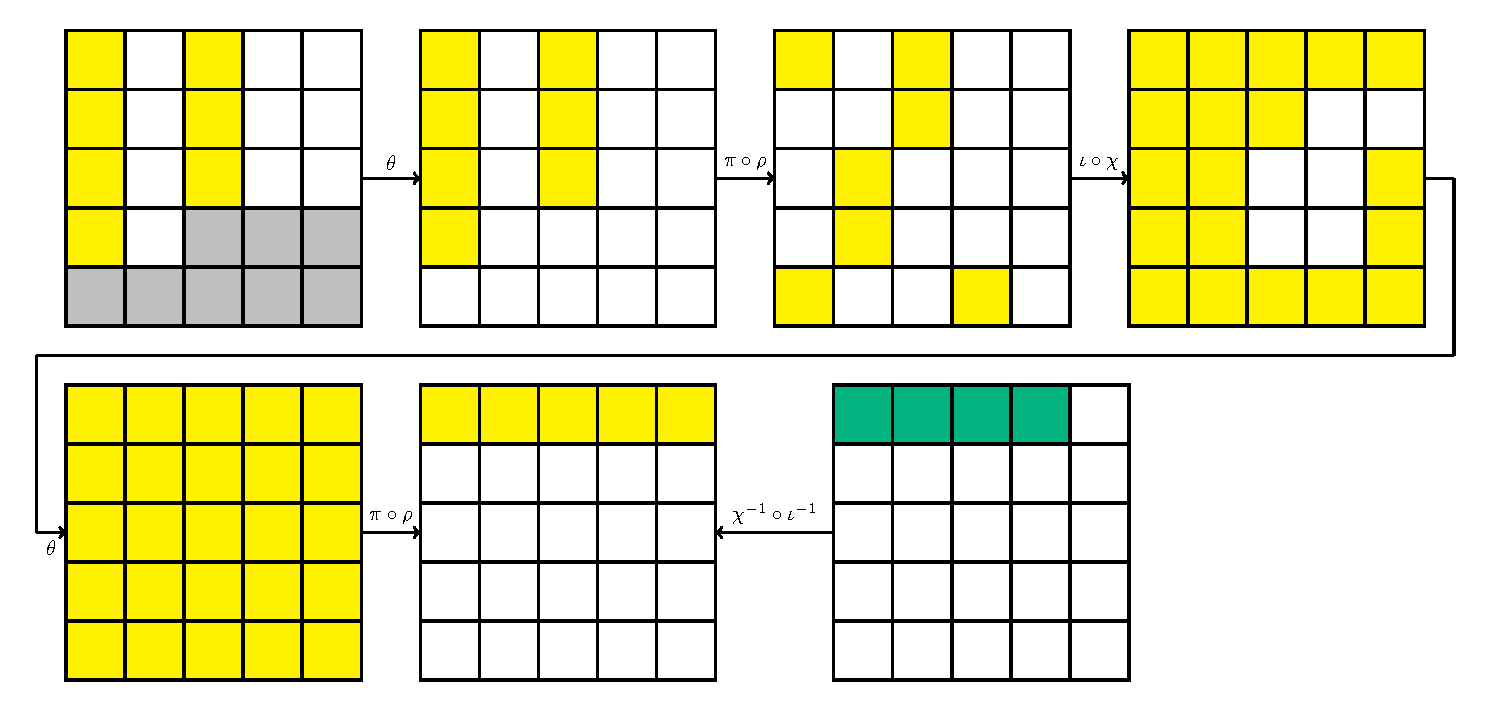
\includegraphics[scale=0.6]{3Rkeccak256.pdf}
        \caption{Preimage Attack on 2-round \KECCAK-$256$}
        \label{fig:3rkeccak256}
\end{figure}

\Keccak-$256$ structure has capacity $c = 256*2 = 8$ lanes and rate$ =  25 - 8 = 17$ lanes. We increase the no. of variable lanes here as compared to \Keccak-$384$ structure, by keeping the lanes $(0,0), (0,1), (0,2), (0,3)$ and $(2,0), (2,1), (2,2)$ as variables in Column $0, 2$ respectively as seen in Figure :~\ref{fig:3rkeccak256}. The yellow colored lanes in the first state represents the variables in rate part of the state and the gray lanes are the $0$ lanes in the capacity part of the state.

To prevent the spread of $\theta$ in first round we need to add constraints :
\begin{enumerate}
\item Keep \[
        A[0,3] = A[0,0] \oplus A[0,1] \oplus A[0, 2] \oplus \alpha_0
    \]
\item \[
        A[2,2] = A[2,0] \oplus A[2,1] \oplus \alpha_2
    \]
\end{enumerate}
Here, $\alpha_0, \alpha_2$ are random constants.
Due to the above constraints the state remains linear and the variables will not spread after application of $\theta$ step mapping as in the second state of the figure. Hence after applying $\iota \circ \chi \circ \pi \circ \rho \circ \theta $ i.e. a round on the initial state, the output state remains linear.

Moving on to the second round, the state is linear even after application of $\pi \circ \rho \circ \theta$, since these step mappings are linear and they don't introduce any non-linear terms. So, input state to $\chi$ step of second round is linear.

On the other hand, for \KECCAK-$256$ we have $d = 256 = 64*4$ i.e. hash value of only 4 lanes. To make it easier to invert the $\chi$ step we assume any random value as value of 5th lane in the hash state. but this will further add more conditions to satisfy those assumed 64 bits for the 5-th lane.
We can directly invert $\iota^{-1}$ from the given hash and then we have $4$ hash lanes then we can apply ~\ref{ob3} to obtain $4$ linear equations on the bits input to $\chi$ for that row. By this we obtain the relations for the input state to the $\chi$ step.

Then we can apply the same technique as mentioned in section 6.3 \cite{guo2016linear} for this structure also. 

If we observe carefully then, each bit of the inverted state is a sum of 11 bits of the output of the second round. Since $\pi \circ \rho$ just permutate the positions of these bits and $\iota$ just add a constant to the first lane, they do not increase the nonlinear terms, and thus we can ignore these step mappings in the last one and a half rounds. As in section 6.3 per equation $(14)$ for $C[x][y][z]$. 

On Expanding it :
    \[
        C[x][y][z] = B[x][y][z] \oplus \oplus_{y' = 0}^{4} B[x-1][y'][z] \oplus \oplus_{y' = 0}^{4} B[x+1][y'][z-1]
    \]
    Open all the expressions and separate two terms $B[x][y][z]$ and $B[x-1][y][z]$ and rest 9 terms remain as it is.
    So, \[ B[x][y][z] \oplus B[x-1][y][z] = (a \oplus c + b) \oplus d
    \]
    Where \[
        a = A[x][y][z], b = A[x + 1][y][z], c = A[x + 2][y][z], d = A[x - 1][y][z]
    \]
    So guessing $b$ and other 9 terms would make $C[x][y][z]$ linear. Hence, We linearize $C[x][y][z]$ by guessing these 10 bits input to step $\chi$. That is, we obtain 11 = 1 + 10 linear equations and match 1 bit of the hash value.
We can match $2\floor*{\frac{t - 5}{8}}$ bits of a given hash value if we have $t$ variables \cite{guo2016linear} and as explained in the preimage attacks section.

For \Keccak-$256$, we started with $7$ lanes variable states in the initial state. After applying conditions to keep $\theta$ as constant we are left with $7 - 2 = 5$ lane variables. Hence $t = 5*64 = 320$ variables.
So the no. of matched bits = $78$, with this we have a complexity gain over brute-force of $2^{78}$
Attack complexity $ = 2^{256 - 78} = 2^{178}$.

This method observes an improvement of $2^{14}$ compared to the attack mentioned in \cite{guo2016linear}.

\section{Preimage attack on 4-round \KECCAK-$224$}
    
    \textbf{Note : } The results under this section are not verified. [TODO]
    
    This is in reference to Guo \etal work "Linear Structures: Applications to Cryptanalysis of Round-Reduced Keccak"~\cite{guo2016linear}. Lets see \KECCAK-$224$ in more detail, so the attack mentioned in section 6.2 has the structure as shown in Figure $14$.
    As seen in Fig. $13, 14$ of section 6.2 of~\cite{guo2016linear}, the attacks for \KECCAK-$256$ and \KECCAK-$224$ resp. These are preimage attacks for 3 rounds where by the method of linear structure they are able to keep the state linear even after the $L$ i.e. $\pi \circ \rho \circ \theta$ part of the third round. So the key point to note here is that the input to the $\chi$ of the third round is linear and this information is being used in the attack described below.
    \begin{figure}
        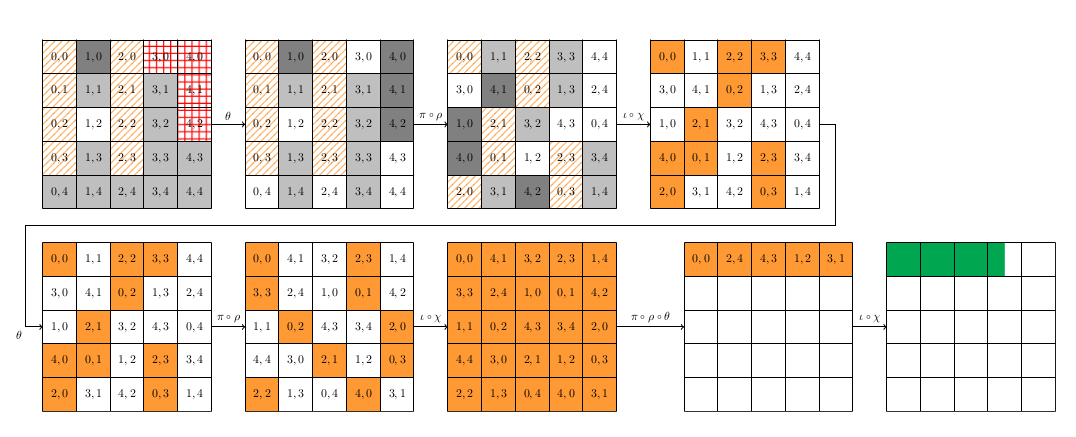
\includegraphics[width=\linewidth]{keccak224.png}
        \caption{Preimage attack on 3-round \KECCAK-$224$~\cite{guo2016linear}}
        \label{fig:keccak224}
    \end{figure}
    Here the input to the step $\chi$ of the third round are all linear variables and its output will be a quadratic state as $\chi$ is a non-linear operation.
    So, if we consider the state input to $\chi$ of third round be $A$, output of $\chi$ be $B$ and output of fourth round $\theta$ be $C$.
    
    Then we have the following relations between $A, B$ and $C$: 
    \[
			B[x][y][z] = A[x][y][z] \oplus (A[x+1][y][z] \oplus 1) \cdot A[x+2][y][z]
		\]
		\[
        C[x][y][z] = B[x][y][z] \oplus \oplus_{y' = 0}^{4} B[x-1][y'][z] \oplus \oplus_{y' = 0}^{4} B[x+1][y'][z-1]
    \]
    We linearize $C[x][y][z]$ by guessing $B[x+1][y'][z-1]$ for all $0 \leq y' \leq 4$ and $B[x-1][y'][z]$ for all $y'$ other than $y$ . These all are 9 guesses.
    The term $C[x][y][z]$ is still quadratic due to $B[x][y][z] \oplus B[x-1][y][z]$, $A[x+1][y][z]$ is a common bit in both $B[x][y][z]$ and $B[x-1][y][z]$. Guessing $A[x+1][y][z]$ makes $B[x][y][z] \oplus B[x-1][y][z]$ term linear. So after guessing $A[x+1][y][z]$ the $C[x][y][z]$ becomes linear and we get one more linear equation, hence a total of $9+1 = 10$ bits are guessed.

    Hence the method for matching hash bits by linearizing the terms corresponding to these hash bits is applied here.
    In this we linearize the output of $\theta$ of 4th round by guessing bits input to $\theta$. We need 10 guesses to match 1-bit.
    
    By this method we obtain $ 1 + 10 $ linear equations by 10 guesses and we are able to match 1 bit of hash value corresponding to $C[x][y][z]$.
    
    Hence we can match $\floor*{ \frac{t}{11} }$ bits of the hash value if we have $t$ variables.
    
    One may think why this method works for \KECCAK-$224$?
    
    For \KECCAK-$224$ we can't invert the hash value through $\chi^{-1}$ as its possible for for \KECCAK-$512$, but we can set up the equations such as $a_0 = b_0$ for $b_1 = 1$ according to (6) equation of Guo \etal paper. ( For inversion of hash through $\chi^{-1}$ we can think of other ideas too, like randomly setting the remaining hash bits in row0, so as to get full row bits or maybe some other method )
    
    The relations obtained after applying invert operation i.e. $\chi^{-1} \circ \iota^{-1}$ on the hash value, each bit of the state just before $\chi$ of the final round is in a way sum of 11 bits of the output of the third round (due to $\theta$). Though positions of these bits will be permuted by $\pi \circ \rho$ and $\iota$ only adds a constant, but these steps don't increase or introduce any non-linear term. So, we can linearize $C[x][y][z]$ and then can match the corresponding hash bit.
    
		For \KECCAK-$224$ we have 127 variables and the no. of matched bits $ = \floor*{ \frac{127}{11} } = 11 $.

    Time Complexity of above method when applied to \KECCAK-$224$ is $ = 2^{224 - 11} = 2^{213}$.
    
    As seen in Improved preimage attacks on 3-round \KECCAK-$384$ and \KECCAK-$512$ by Guo \etal in section 6.3 . So instead of choosing linear independent bits for linearizing, if we choose terms such that when guesses are made to linearize them, then it will also decrease the no. of guesses required for some other bits. So it will be possible to further decrease the complexity if we choose such dependent variables. Since there will be more degrees of freedom for guessing more linear combinations to match more bits of the hash value. So we start with following two equations, $B$ represents the state after third round $\chi$ ,
	\[
		B[x][y][z] = A[x][y][z] \oplus (A[x+1][y][z] \oplus 1) \cdot A[x+2][y][z]
	\] and
	\[
		B[x-1][y][z] = A[x-1][y][z] \oplus (A[x][y][z] \oplus 1) \cdot A[x+1][y][z]
	\]

	By guessing $A[x+1][y][z]$ we make both of the above equations linear.
	
	Hence we guess for $0 \leq y \leq 4$ $A[x+1][y][z]$. Similarly for $B[x+1][y][z-1], B[x+2][y][z-1]$ we guess $0 \leq y \leq 4$ $A[x+3][y][z-1]$. 
	\[
        C[x][y][z] = B[x][y][z] \oplus \oplus_{y' = 0}^{4} B[x-1][y'][z] \oplus \oplus_{y' = 0}^{4} B[x+1][y'][z-1]
    \] and 
	\[
        C[x+1][y+1][z] = B[x+1][y+1][z] \oplus \oplus_{y' = 0}^{4} B[x][y'][z] \oplus \oplus_{y' = 0}^{4} B[x+2][y'][z-1]
    \]

    These 10 bits are guessed not only make $C[x][y][z]$ linear, but $C[x+1][y+1][z]$ has only one quadratic term $B[x+1][y+1][z]$ left and after guessing that $C[x+1][y+1][z]$ is also linear. 
    
    We can match 2 bits by setting up 13 (10 + 1 + 2) linear equations. 
    
    Then we consider another two equations :
    
    	\[
        C[x + 2][y+2][z-1] = B[x + 2][y+2][z-1] \oplus \oplus_{y' = 0}^{4} B[x+1][y'][z-1] \oplus \oplus_{y' = 0}^{4} B[x+3][y'][z-2]
    \] and 
		\[
        C[x+3][y+3][z-1] = B[x+3][y+3][z-1] \oplus \oplus_{y' = 0}^{4} B[x+2][y'][z-1] \oplus \oplus_{y' = 0}^{4} B[x+4][y'][z-2]
    \]
    
    Here we can set up another 8 linear equations and match two more bits of the hash value by guessing 6 more bits. So in general, if there are $t$ variables then we can match $2\floor*{\frac{t-5}{8}}$.
    
    So, if we apply the same technique to 4 rounds of \KECCAK-$224$, \KECCAK-$256$
    Then we have 127 and 64 variables respectively, we can match $2\floor*{\frac{t-5}{8}}$ bits of a hash value if we have $t$ variables.
    For Keecak-224 : matched bits $= 30$ for $t = 127$.
    
    Time Complexity : $2^{224 - 30} = 2^{194}$ and similarly for \KECCAK-$256$, Time complexity $=2^{256 - 14} = 2^{242}$

